\documentclass[12pt,a4paper]{report}
%%%%%%%%%%%%%%%%%%%%%%%%%%%%%%%%%%%%%%%%%%%%%%%%%%%%%%%%%%%%%%%%%
%TCIDATA{OutputFilter=LATEX.DLL}
%TCIDATA{Version=5.50.0.2934}
%TCIDATA{<META NAME="SaveForMode" CONTENT="1">}
%TCIDATA{BibliographyScheme=Manual}
%TCIDATA{<META NAME="DocumentShell" CONTENT="Scientific WorkPlace\LaTeX Report">}
%TCIDATA{Language=Turkish}
%TCIDATA{CSTFile=LaTeX Report.cst}
%TCIDATA{PageSetup=72,72,72,72,0}
%%%%%%%%%%%%%%%%%%%%%%%%%%%%%%%%%%%%%%%%%%%%%%%%%%%%%%%%%%%%%%%%%
\usepackage[utf8]{inputenc}
\usepackage[T1]{fontenc}
\usepackage[shorthands=off,turkish]{babel}
\usepackage{amsmath,amssymb,amsthm}
\usepackage{graphicx}
\usepackage{float}
\usepackage{booktabs}
\usepackage{pdflscape}
\usepackage{caption}
\usepackage{subcaption}
\graphicspath{{./fig/}{fig/}}
\providecommand{\parencite}[1]{(#1)}
\providecommand{\textcite}[1]{#1}
\providecommand{\sekilnotu}[1]{\par\small #1}
\providecommand{\tablonotu}[1]{\par\small #1}
\providecommand{\subsubsubsection}[1]{\paragraph{#1}\mbox{}\\}
\begin{document}
%%%%%%%%%%%%%%%%%%%%%%%%%%%%%%%%%%%%%%%%%%%%%%%%%%%%%%%%%%%%%%%%%
\chapter{MATERYAL VE METOT}\label{ch:fp}
%%%%%%%%%%%%%%%%%%%%%%%%%%%%%%%%%%%%%%%%%%%%%%%%%%%%%%%%%%%%%%%%%

\section{Ara\c{s}t\i{}rma Materyali}

Bu b\"{o}l\"{u}mde \c{c}al\i{}\c{s}mada kullan\i{}lan veri, deney materyali, yaz\i{}l\i{}m, donan\i{}m, saha bilgisi veya belge kaynaklar\i{} tan\i{}t\i{}l\i{}r. Materyalin nas\i{}l elde edildi\u{g}i, hangi kapsama sahip oldu\u{g}u ve hangi s\i{}n\i{}rl\i{}l\i{}klar\i{} i\c{c}erdi\u{g}i a\c{c}\i{}klanmal\i{}d\i{}r.

\subsection{Veri Kaynaklar\i{}}

Veri kaynaklar\i{} yaz\i{}l\i{}rken tarih aral\i{}\u{g}\i{}, \"{o}rneklem b\"{u}y\"{u}kl\"{u}\u{g}\"{u}, \"{o}l\c{c}\"{u}m birimleri ve veri se\c{c}im \"{o}l\c{c}\"{u}tleri belirtilir. Gerekirse veri haz\i{}rlama s\"{u}reci a\c{s}amalar halinde verilebilir.

\begin{figure}[!ht]
 \centering
 
\includegraphics[width=230pt,keepaspectratio=true]{./fig/sekil3}
 \vspace*{4mm}
 \caption[K\i{}sa \c{s}ekil a\c{c}\i{}klamas\i{}]{Uzun \c{s}ekil a\c{c}\i{}klamas\i{}nda listenin k\i{}sa s\"{u}r\"{u}m\"{u} kullan\i{}labilir}
 \label{fig:3-1-1}
\end{figure}

\c{S}ekil~\ref{fig:3-1-1}, veri veya y\"{o}ntem ak\i{}\c{s}\i{}n\i{} g\"{o}stermek i\c{c}in kullan\i{}labilecek bir g\"{o}rsel \"{o}rne\u{g}idir.

\section{Y\"{o}ntem}

Y\"{o}ntem k\i{}sm\i{}, \c{c}al\i{}\c{s}man\i{}n tekrarlanabilmesini sa\u{g}layacak ayr\i{}nt\i{}da yaz\i{}lmal\i{}d\i{}r. Kullan\i{}lan analiz ad\i{}mlar\i{}, yaz\i{}l\i{}m ayarlar\i{}, varsay\i{}mlar ve de\u{g}erlendirme \"{o}l\c{c}\"{u}tleri burada verilir.

\subsection{Model Kurulumu}

Model veya analiz yakla\c{s}\i{}m\i{} a\c{c}\i{}klan\i{}rken temel denklemler numaraland\i{}r\i{}labilir. Denklem~\ref{eq:3-1}, zaman serisi benzeri bir g\"{o}sterim i\c{c}in \"{o}rnek olarak verilmi\c{s}tir.

\begin{equation}
\label{eq:3-1}
   y_{t}  \equiv \phi_{1} y_{t-1} + \epsilon_{t}
\end{equation}

Denklemden sonra sembollerin anlam\i{} ve modeldeki rolleri metin i\c{c}inde a\c{c}\i{}klanmal\i{}d\i{}r. Daha uzun denklemler gerekiyorsa sat\i{}r k\i{}r\i{}mlar\i{} okunabilirli\u{g}i bozmayacak bi\c{c}imde d\"{u}zenlenmelidir. Birden fazla sat\i{}rda verilen denklemlerde numara son sat\i{}r hizas\i{}nda yer almal\i{}d\i{}r; Denklem~\ref{eq:3-2} bu kullan\i{}ma \"{o}rnektir.

\begin{align}
\widehat{y}_{t}
  &= \beta_{0} + \beta_{1}x_{1t} + \beta_{2}x_{2t} \notag\\
  &\quad + \beta_{3}x_{3t} + \varepsilon_{t}
  \label{eq:3-2}
\end{align}

\subsection{Analiz S\"{u}reci}

Analiz s\"{u}reci; \"{o}n i\c{s}leme, modelleme, do\u{g}rulama ve yorumlama ad\i{}mlar\i{}ndan olu\c{s}abilir. Her ad\i{}m\i{}n amac\i{} ve \c{c}al\i{}\c{s}madaki kar\c{s}\i{}l\i{}\u{g}\i{} a\c{c}\i{}k\c{c}a belirtilmelidir.

\begin{figure}[!ht]
 \centering
 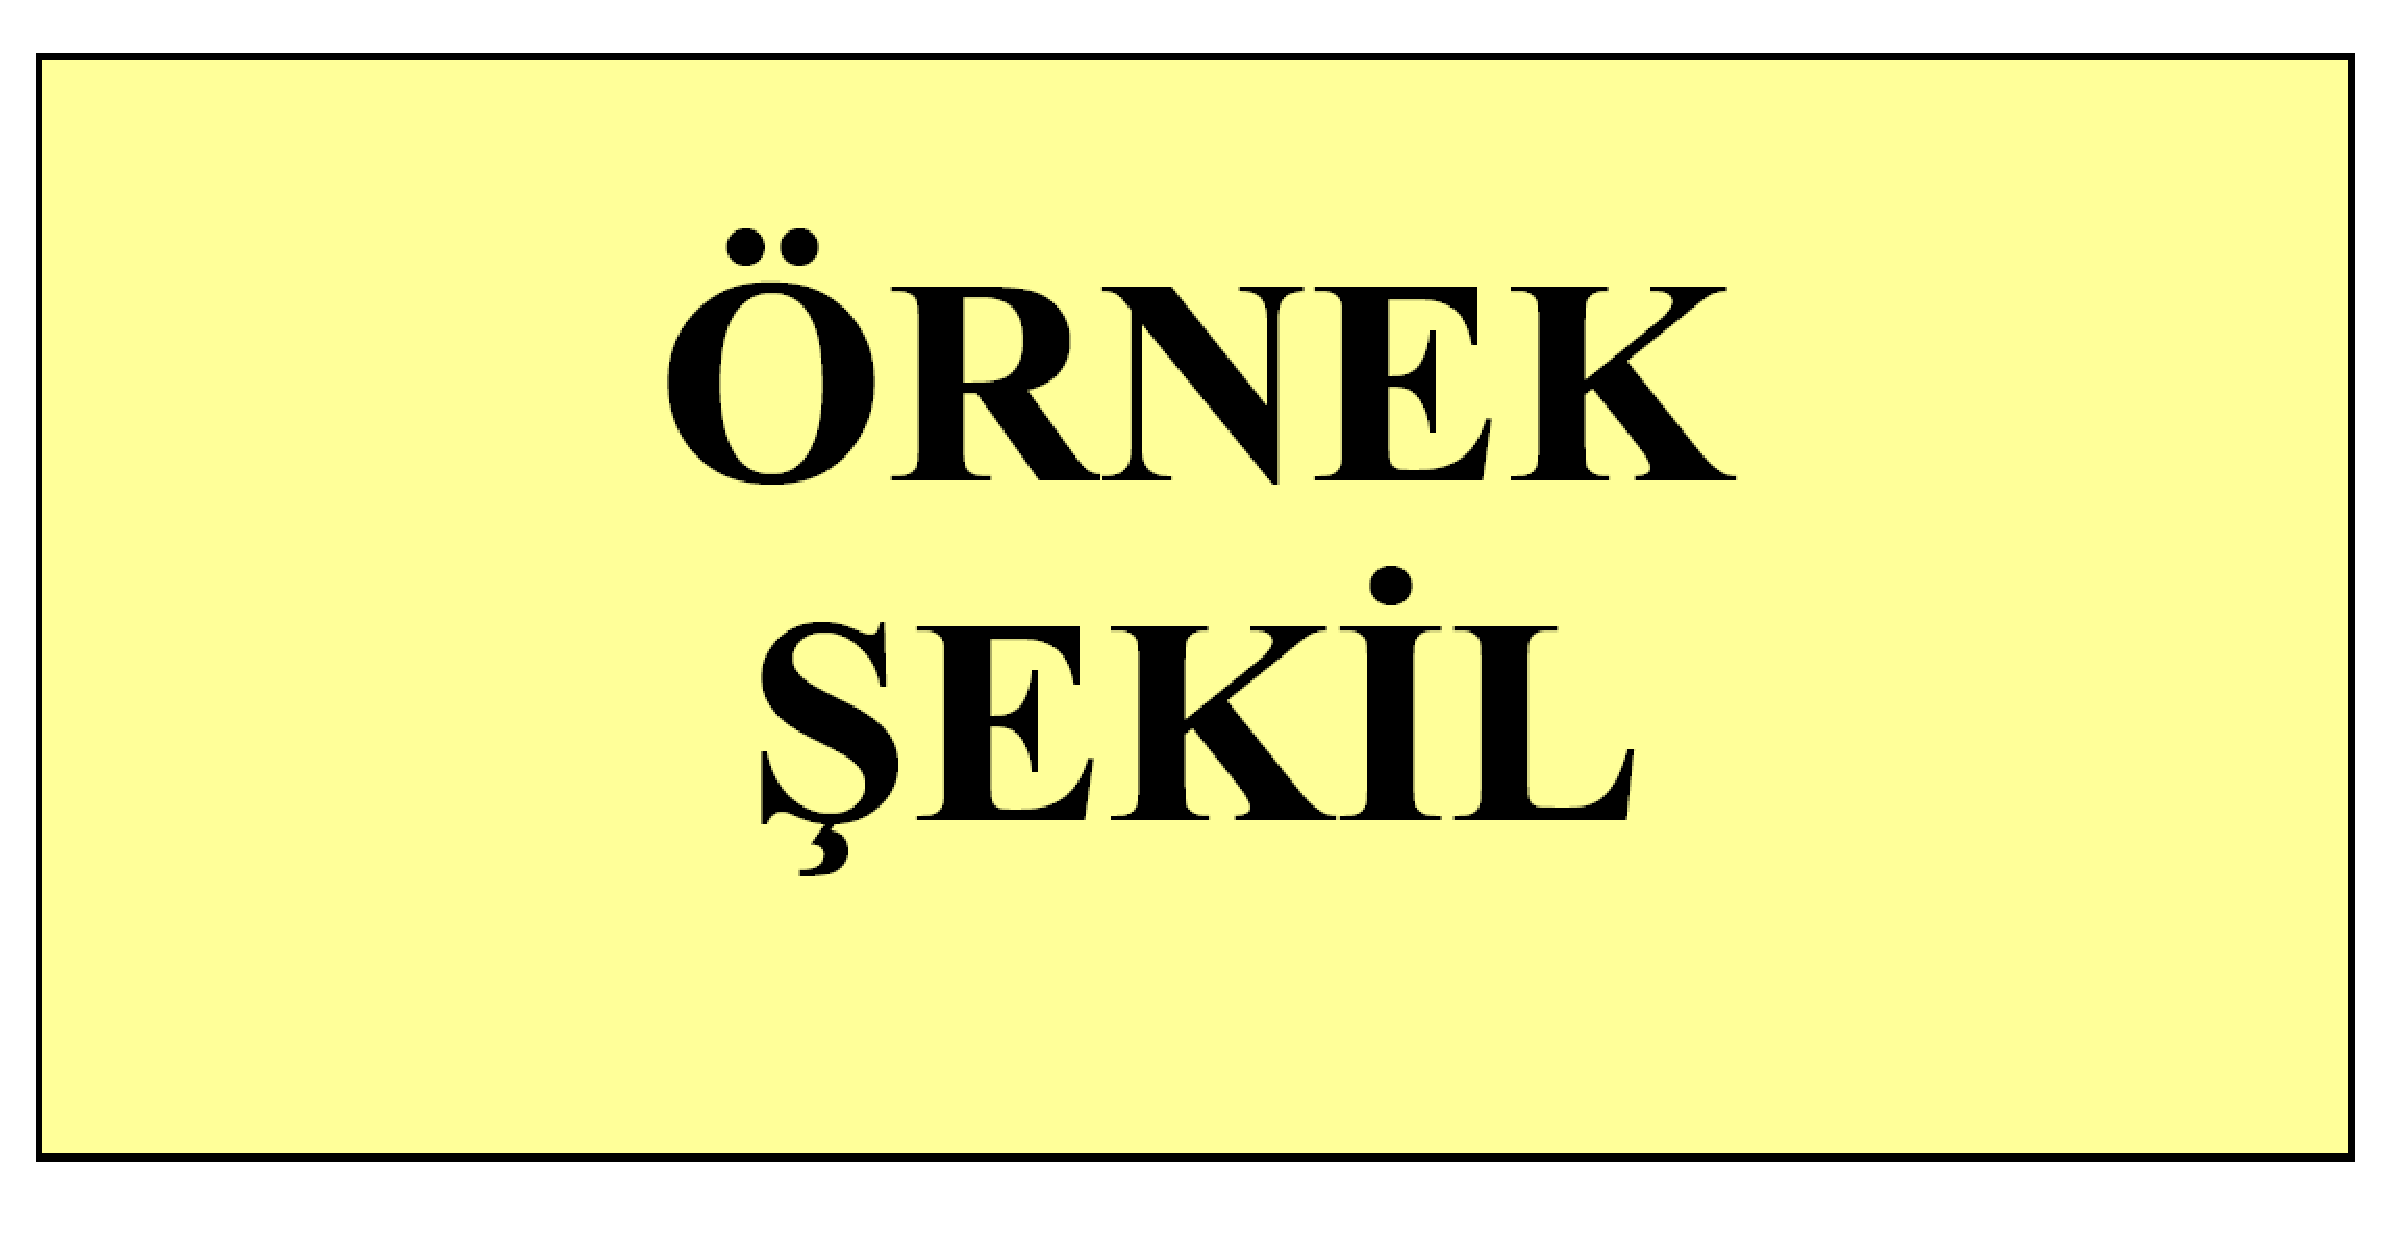
\includegraphics[width=230pt,keepaspectratio=true]{./fig/sekil4}
 \vspace{4mm}
 \caption{\c{C}ok sat\i{}rl\i{} \c{s}ekil a\c{c}\i{}klamalar\i{}nda hizalama \"{o}rne\u{g}i}
 \label{fig:3-1-3}
\end{figure}

\c{S}ekil~\ref{fig:3-1-3}'de y\"{o}ntemin i\c{s} ak\i{}\c{s}\i{} g\"{o}sterilmektedir. \c{S}ekil a\c{c}\i{}klamalar\i{} nokta ile bitirilmemeli ve metin i\c{c}inde ilgili \c{s}ekle mutlaka g\"{o}nderme yap\i{}lmal\i{}d\i{}r.

\section{Yatay Tablo ve \c{S}ekil \"{O}rnekleri}

Sayfaya s\i{}\u{g}mayan tablo veya \c{s}ekiller yatay olarak verilebilir. Yatay kullan\i{}m zorunlu olmad\i{}k\c{c}a tercih edilmemeli, kullan\i{}ld\i{}\u{g}\i{}nda ba\c{s}l\i{}k ve sayfa numaras\i{} yerle\c{s}imi kontrol edilmelidir.

\begin{landscape}
\begin{table}[!ht]
\caption{Yatay sayfada tablo \"{o}rne\u{g}i}
\centering
\begin{tabular}{cccccc}
\hline\hline
De\u{g}i\c{s}ken & A & B & C & D & E \\
\hline
\"{O}rnek 1 & 12 & 18 & 24 & 31 & 35 \\
\"{O}rnek 2 & 14 & 21 & 26 & 33 & 39 \\
\"{O}rnek 3 & 16 & 23 & 29 & 37 & 42 \\
\hline
\end{tabular}
\label{table:landscape_table1}
\end{table}
\end{landscape}

Tablo~\ref{table:landscape_table1}, geni\c{s} i\c{c}erikli tablolar\i{}n yatay sayfada nas\i{}l verilebilece\u{g}ini g\"{o}steren bir \"{o}rnektir.
\end{document}
